\documentclass{beamer}
\usetheme{Berlin}
\usecolortheme{beaver}
\usepackage[utf8]{inputenc}
\usepackage[czech]{babel}
\usepackage{hyperref}

\setbeamerfont{page number in head/foot}{size=\small}
\setbeamertemplate{footline}[frame number]


\title
{Diplomová práce}
\subtitle{Inteligentní zabezpečovací systém garáže: nadřazený systém }
\author
{Ondřej Červenka \\ Vedoucí: Ing. Martin Daňhel}
\institute
{
  České vysoké učení technické v Praze\\
  Fakulta informačních technologií
}
\date{2018}

\begin{document}
  \frame{\titlepage}
  \begin{frame}
    \frametitle{Cíl práce}

    Cílem práce bylo navrhnout a implementovat systém určený k zabezpečení garážového komplexu. Systém sbírá data od podřízených systémů monitorujících stav jednotlivých garážích.

    % tady strucne popsat ten podrizenej system, tj zarizeni, ktery je v ty garazi a ma naky senzory kterejma monitoruje jeji stav

    % pak prejit hned na ten dalsi slajd s tim vobrazkem, rict ze to teda vypada takhle

  \end{frame}

  \begin{frame}
    \frametitle{Návrh systému}

    \begin{figure}
        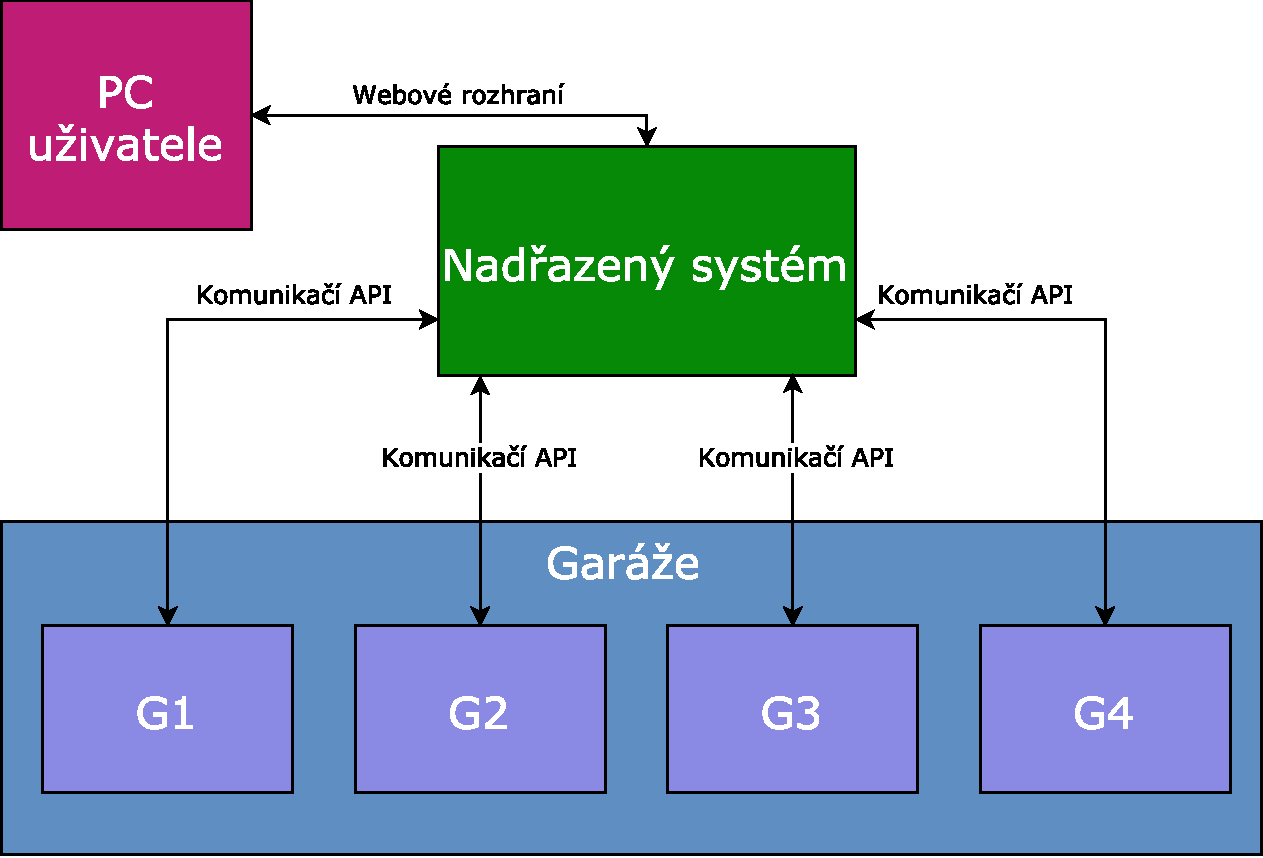
\includegraphics[scale=0.3]{../images/basic_struct.pdf}
        \caption{Základní struktura systému.}
      \end{figure}

      % rict ze ty podrizeny systemy komunikujou s nadrazenym
      % na zaklade udalosti zasilanejch pres ten komunikacni kanal (api)
      % popsat udalost (priklad)
  \end{frame}

  \begin{frame}
    \frametitle{Návrh systému}

      % tady uz bude popsana zakladni strukura toho systemu, takze muzu zacit popisovat konkretni pozadavky, ty dalsi slajdy pak vychazej z tech pozadavku

      % zacit to tak, ze konkretni pozadavky na system byly takovyhle

      Požadavky na systém:

      \begin{itemize}
        \item Komunikace s podřízenými systémy pomocí WiFi nebo Ethernetu.
        \item Webové uživatelské rozhraní pro správu.
        \item Reakce na události zaslané podřízenými systémy.
        \item Možnost provozu na jednodeskovém počítači (omezený HW). % tady rict ze sme chteli uceleny zarizeni
      \end{itemize}
  \end{frame}

  \begin{frame}
    \frametitle{Návrh systému}
    \framesubtitle{Komunikační protokol}

    Zkoumány byly protokoly HTTPS a MQTT:

    \begin{itemize}
      \item HTTPS: 
      \begin{itemize}
        \item Jeden server pro webové rozhraní a API.
        \item Snazší implementace.
        \item Široká podpora.
      \end{itemize}
      \item MQTT:
      \begin{itemize}
        \item Složitější implementace.
      \end{itemize}
    \end{itemize}

    Pro implementaci systému byl zvolen protokol HTTPS.

    % rict ze api primarne slouzi k zasilani udalosti vod podrizenejch systemu
    % tady říct, že to api slouží i k registraci/autorizaci systémů pomocí api klíčů.
    % taky rict ze duvody pro tuhle volbu bylo: jeden web server pro api i rozhrani, jednoduchost implementace

  \end{frame}

  \begin{frame}
    \frametitle{Návrh systému}
    \framesubtitle{Webové rozhraní}

    Webové rozhraní je určeno ke správě podřízených systémů a umožňuje:

    \begin{itemize}
      \item Registraci nových systému.
      \item Zobrazení zaznamenaných událostí.
      \item Editaci záznamu garáže (telefonní číslo, popis atp.).
      \item Změnu uživatelského nastavení.
    \end{itemize}

    Přístup do rozhraní je zabezpečen heslem.
    
  \end{frame}

  \begin{frame}
    \frametitle{Návrh systému}
    \framesubtitle{Webové rozhraní}

    % jen rict ze tohle je ukazka zobrazeni konkretni garaze, a ze teda vidime ty zaznamenany udalosti

    \begin{figure}
        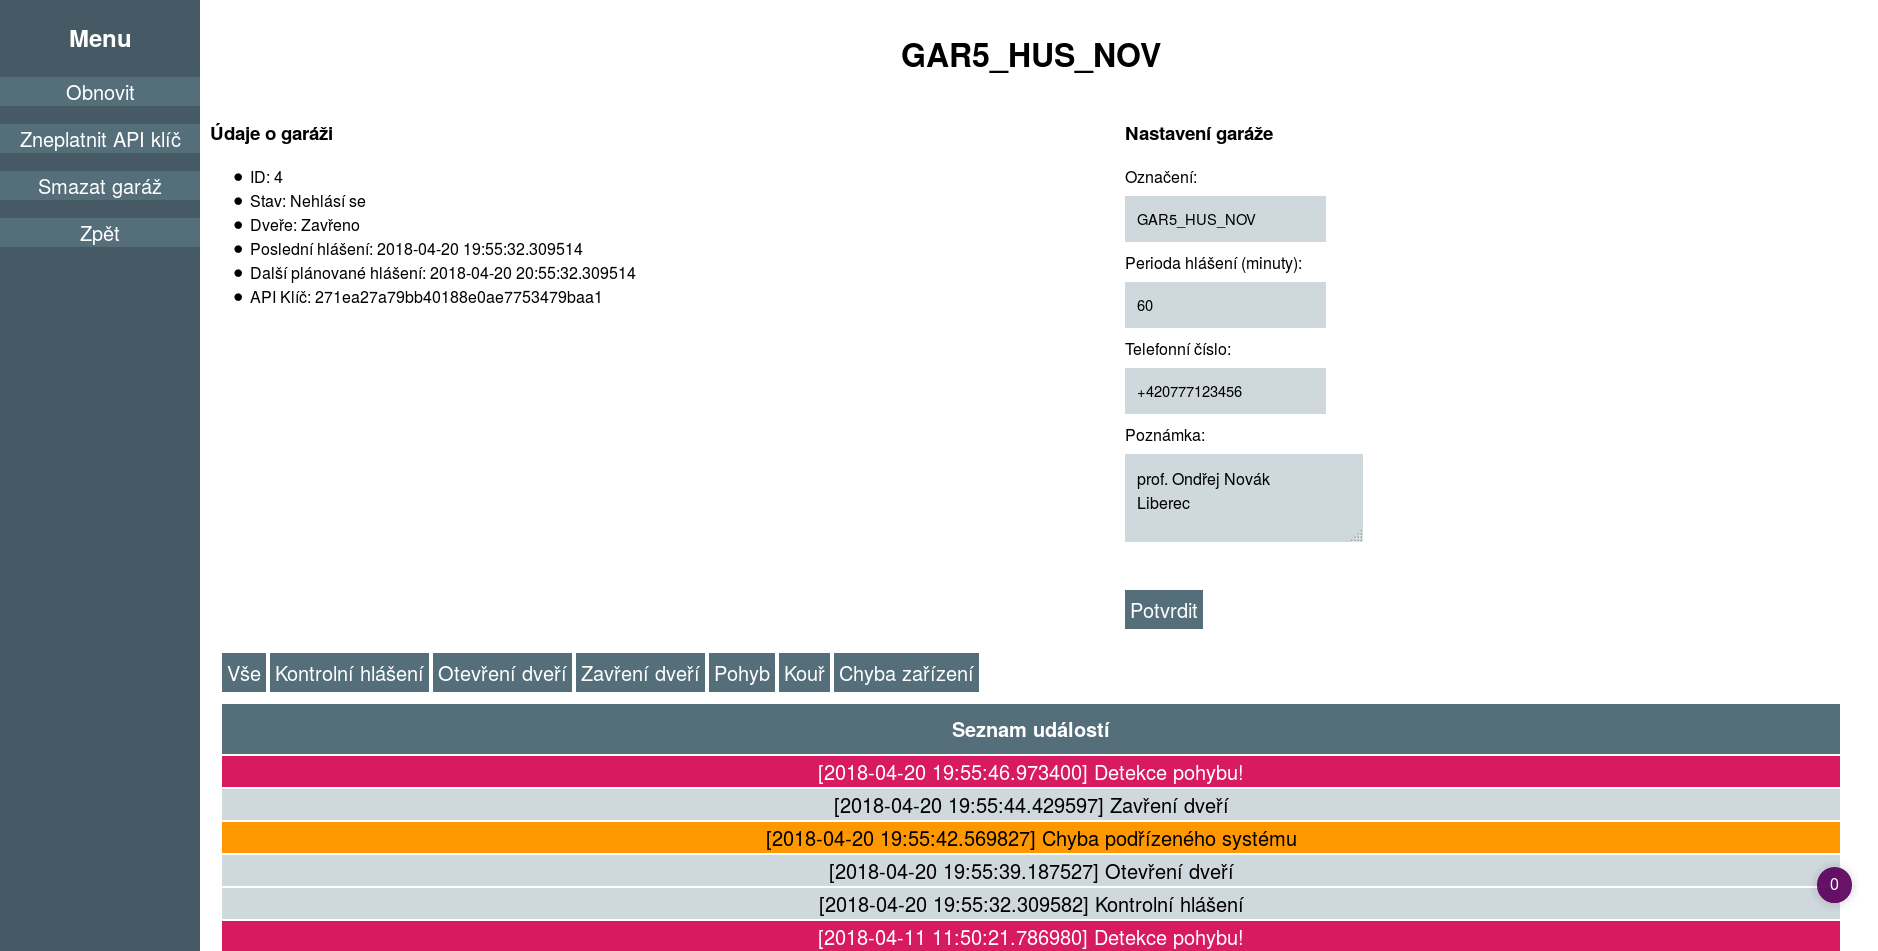
\includegraphics[scale=0.161]{../images/webp.png}
        \caption{Webové rozhraní systému.}
      \end{figure}
    
  \end{frame}

  \begin{frame}
    \frametitle{Návrh systému}
    \framesubtitle{Reakce na události}

    Zasílání upozornění v případě poplachu:

    \begin{figure}
        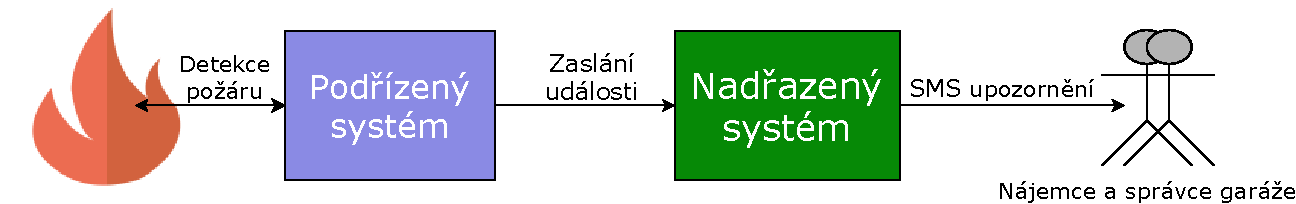
\includegraphics[scale=0.45]{../images/alert.pdf}
    \end{figure}

    Zkoumané metody:

    \begin{itemize}
      \item E-mail -- pomocí Google GMail.
      \item SMS:
      \begin{itemize}
        \item služba Twilio,
        \item \textbf{GSM modul}. 
      \end{itemize}
    \end{itemize}

    % popsat ten flow toho posilani upozorneni jak je na tim vobrazku, tj. tu situaci ktera k tomu vede
    % rict ze spravci a najemci prijdou jiny smsky
    % strucne rict ze sem zkoumal tyhle metody a nakonec zvolil gsm modul (jednoduchost, staci simkarta)

  \end{frame}

  \begin{frame}
    \frametitle{Implementace}

    \begin{itemize}
      \item Programovací jazyk Python 3,
      \begin{itemize}
        \item webový framework Flask,
      \end{itemize}
      \item databázový systém SQLite 3,
      \item program Gammu pro ovládání GSM modulu.
    \end{itemize}

    % rict ze implementace byla primarne delana pro rpi, ale ze to de pouzit na v podstate libovolny platforme s temahle vecma

  \end{frame}

  \begin{frame}
    \frametitle{Testování systému}

    \begin{itemize}
      \item Automatizované testy. % unit testy, dulezity pro dalsi rozsirovani
      \item Manuálni testy. % u tech smsek/gsm modulu
      \item Testovací nasazení.
      \item Simulátor podřízeného systému.
    \end{itemize}

  \end{frame}

  \begin{frame}
    \frametitle{Nasazení systému na Raspberry Pi}

    \begin{figure}
        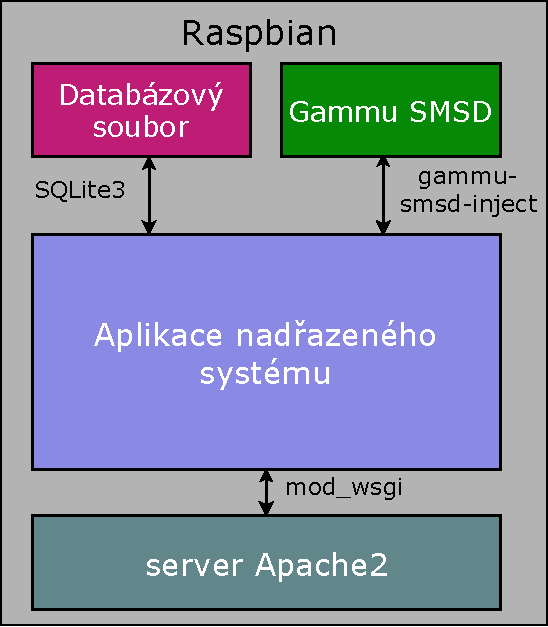
\includegraphics[scale=0.55]{../images/sw_block.pdf}
        \caption{Blokové schéma nasazeného systému.}
      \end{figure}

      % tady znova zminit, ze ta implementace je na tomhle vlastne nezavisla
      % tj by tam mohlo bejt klidne treba mysql nebo jinej operacni system atd...

  \end{frame}

  \begin{frame}
    \frametitle{Závěr}

    Výsledkem práce je zařízení (nadřazený systém) založené na Raspberry Pi, které umožňuje sběr dat od podřízených systémů. Nadřazený systém je možno spravovat pomocí webového rozhraní.

    \vspace{0.5cm}

    Systém byl vyvíjen především pro nasazení na Raspberry Pi, je však možné jej použít na množství dalších platforem. 

  \end{frame}

  \begin{frame}[noframenumbering]
    \frametitle{Otázky oponenta}

    Bylo by možné upravit webové rozhraní tak, aby podporovalo více uživatelů s různými právy? 

    Např. nájemce jedné z garáží by mít možnost sledovat události ve své garáži, případně upravovat telefonní číslo apod.

  \end{frame}

  \begin{frame}[noframenumbering]
    \frametitle{Otázky oponenta}
    \framesubtitle{Přidání zákaznických účtů}

    Úpravy současného kódu:

    \begin{itemize}
      \item Funkce zajišťující přihlášení: uložení informací o účtu. % jestli je ucet admin nebo zakaznik, ktery garaze k uctu patrej atd.
      \item Funkce ověřující přihlášení: kontrola uložených informací.
      % jestli se zakaznik nesnazi zobrazit garaze ktery mu nepatrej, nebo jestli nezkousi smazat garaz atd.
      \item Drobné úpravy uživatelského rozhraní. % odstraneni prislusnejch tlacitek (mazani garaze) pri prihlaseni jako zakaznik. 
    \end{itemize}

    Nové funkce:

    \begin{itemize}
      \item Registrace zákaznických účtů. % pres admina, urci ktery garaze k uctu patrej
      \item Správa zákaznických účtů. % mazani, zmeny najemcu garazi
    \end{itemize}

  \end{frame}

\end{document}
